\documentclass[a4paper]{article}
\usepackage[dvipsnames]{xcolor}
\usepackage[top=70pt,bottom=70pt,left=48pt,right=46pt]{geometry}
\definecolor{header}{RGB}{92,184,92}
\definecolor{defenition}{RGB}{217,83,79}
\definecolor{main_title}{RGB}{66,139,202}
\definecolor{sub_header}{RGB}{91,192,222}
\usepackage[english, russian]{babel}
\usepackage[utf8]{inputenc}
\usepackage{amsmath}
\usepackage{listings}
\usepackage{graphicx}
\usepackage{amsmath}
\usepackage{epigraph} 
\title{\textcolor{main_title}{Предсказание характеристик мемристора в рамках компактной модели по предыдущим циклам переключения}}
\author{Шмаков Владимир Евгеньевич - ФФКЭ гр. Б04-105}






\begin{document}
\maketitle

\epigraph{Такой вещи, как идеальный текст, не существует. Как не существует идеального отчаяния... \newline
Какой текст может написать человек, посреди ночи роющийся в холодильнике на спящей кухне? Только вот такой и может.}{\textit{Харуки Мураками - <<Слушай песню ветра>>}}
\blindtext


\section*{\textcolor{header}{Аннотация}}

\textcolor{defenition}{Мемристор} - устройство, проводимость которого зависит от протекшего через него заряда. При нулевой силе тока сопротивление мемристора остаётся неизменным. 




Моделирование устройства можно провести решением физических уравнений(различных уравнений переноса). 
Либо при помощи \textcolor{defenition}{компактных моделей} - квази-физических уравнений несложно решающихся вычислительными методами.



Современные мемристоры обладают нелинейной вольт-амперной характеристикой. 
Сложность задачи моделирования обусловлена изменением характеристики по ходу эксплуатации устройства.

В данной статье рассматривается решение задачи предсказания характеристик мемристора в рамках компактной модели по предыдущим циклам переключения. <<Нестрогие>> комактные модели обладают значительно меньшими вычислительными затратами по сравнениею со строгими физическими уравнениями переноса. Помимо этого, компактные модели содержат физические характеристики мемристора. Предсказывая параметры компактной модели мемристора по ВАХ можно узнать его строгие характеристики. Составив временной ряд из найденных характеристик сможем предсказать поведение мемристора во времени. 

\section*{\textcolor{header}{Цель}}


Целью данной работы является создание модели, предсказывающей поведение мемристора во времени. 
В качестве модели мемристора используется компактная модель. 
Для оптимизации параметров компактной модели используются алгоритмы глубокого обучения.

\section*{\textcolor{header}{Актуальность}}

\begin{minipage}[l]{0.5\textwidth}
    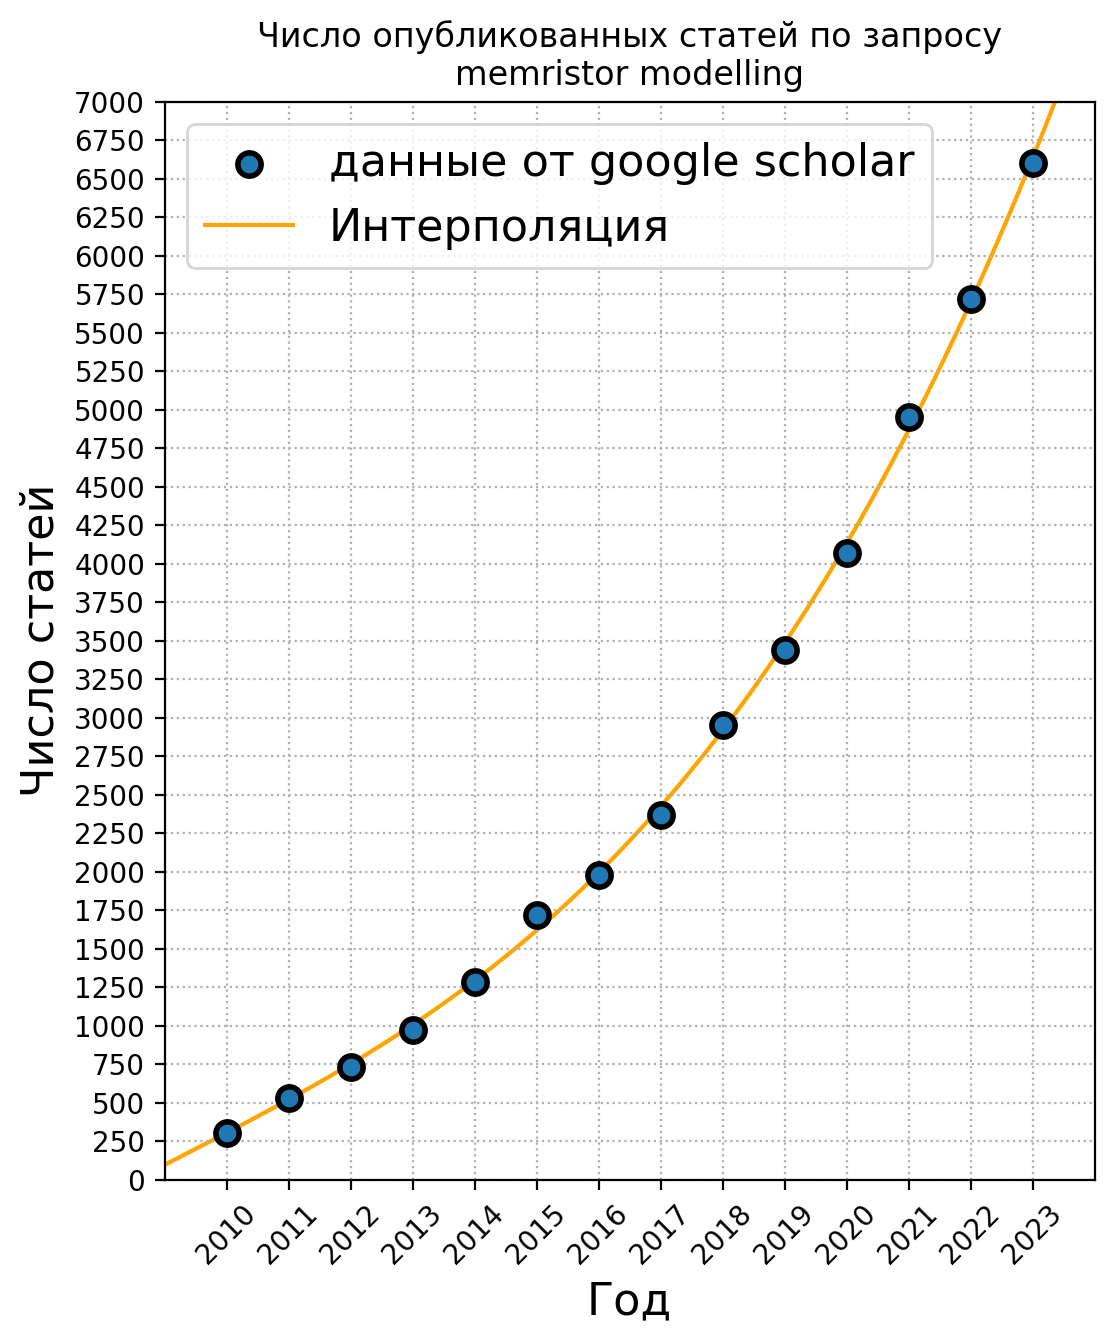
\includegraphics[width=0.9\textwidth]{actuality.png}
\end{minipage}
\begin{minipage}[r]{0.5\textwidth}
    Как видно на графике слева,  задача моделирования мемристора является актуальной. 
    Количество публикаций на эту тему экспоненциально растет.

    Тут добавить сравнение с другими авторами... Чем мы лучше... Но пока прочитано  мало статей и написано  мало кода.
\end{minipage}

\section*{\textcolor{header}{Задачи}}

\begin{enumerate}
    \item Численно решить компактные уравнения, моделирующие поведение мемристора.
    \item Проведя сравнение, выбрать наилучшую компакнтую модель
    \item Выбрать архитектуру нейронной сети, решающей задачу предсказания параметров компактной модели по экспериментальной ВАХ.
    \item Выбрать архитектуру нейронной сети, способной предсказывать изменения параметров компактной модели во времени
    \item Оценить точность моделей
    \item Промоделировать некоторые схемы с использованием мемристоров(например схему нейрона)
    
\end{enumerate}
   





\end{document}
